\usetikzlibrary{matrix}

\colorlet{helpful}{lime!70}
\colorlet{harmful}{red!30}
\colorlet{internal}{yellow!20}
\colorlet{external}{cyan!30}
\colorlet{S}{helpful!50!internal}
\colorlet{W}{harmful!50!internal}
\colorlet{O}{helpful!50!external}
\colorlet{T}{harmful!50!external}

\newcommand{\texta}{Helpful\\ \tiny (to achieve the objective)\par}
\newcommand{\textb}{Harmful\\ \tiny (to achieve the objective)\par}
\newcommand{\textcn}{Internal origin\\ \tiny (product\slash company attributes)\par}
\newcommand{\textdn}{External origin\\ \tiny (environment\slash market attributes)\par}

\newcommand{\back}[1]{\fontsize{60}{70}\selectfont #1}
%\noindent\resizebox{\textwidth}{!}{
	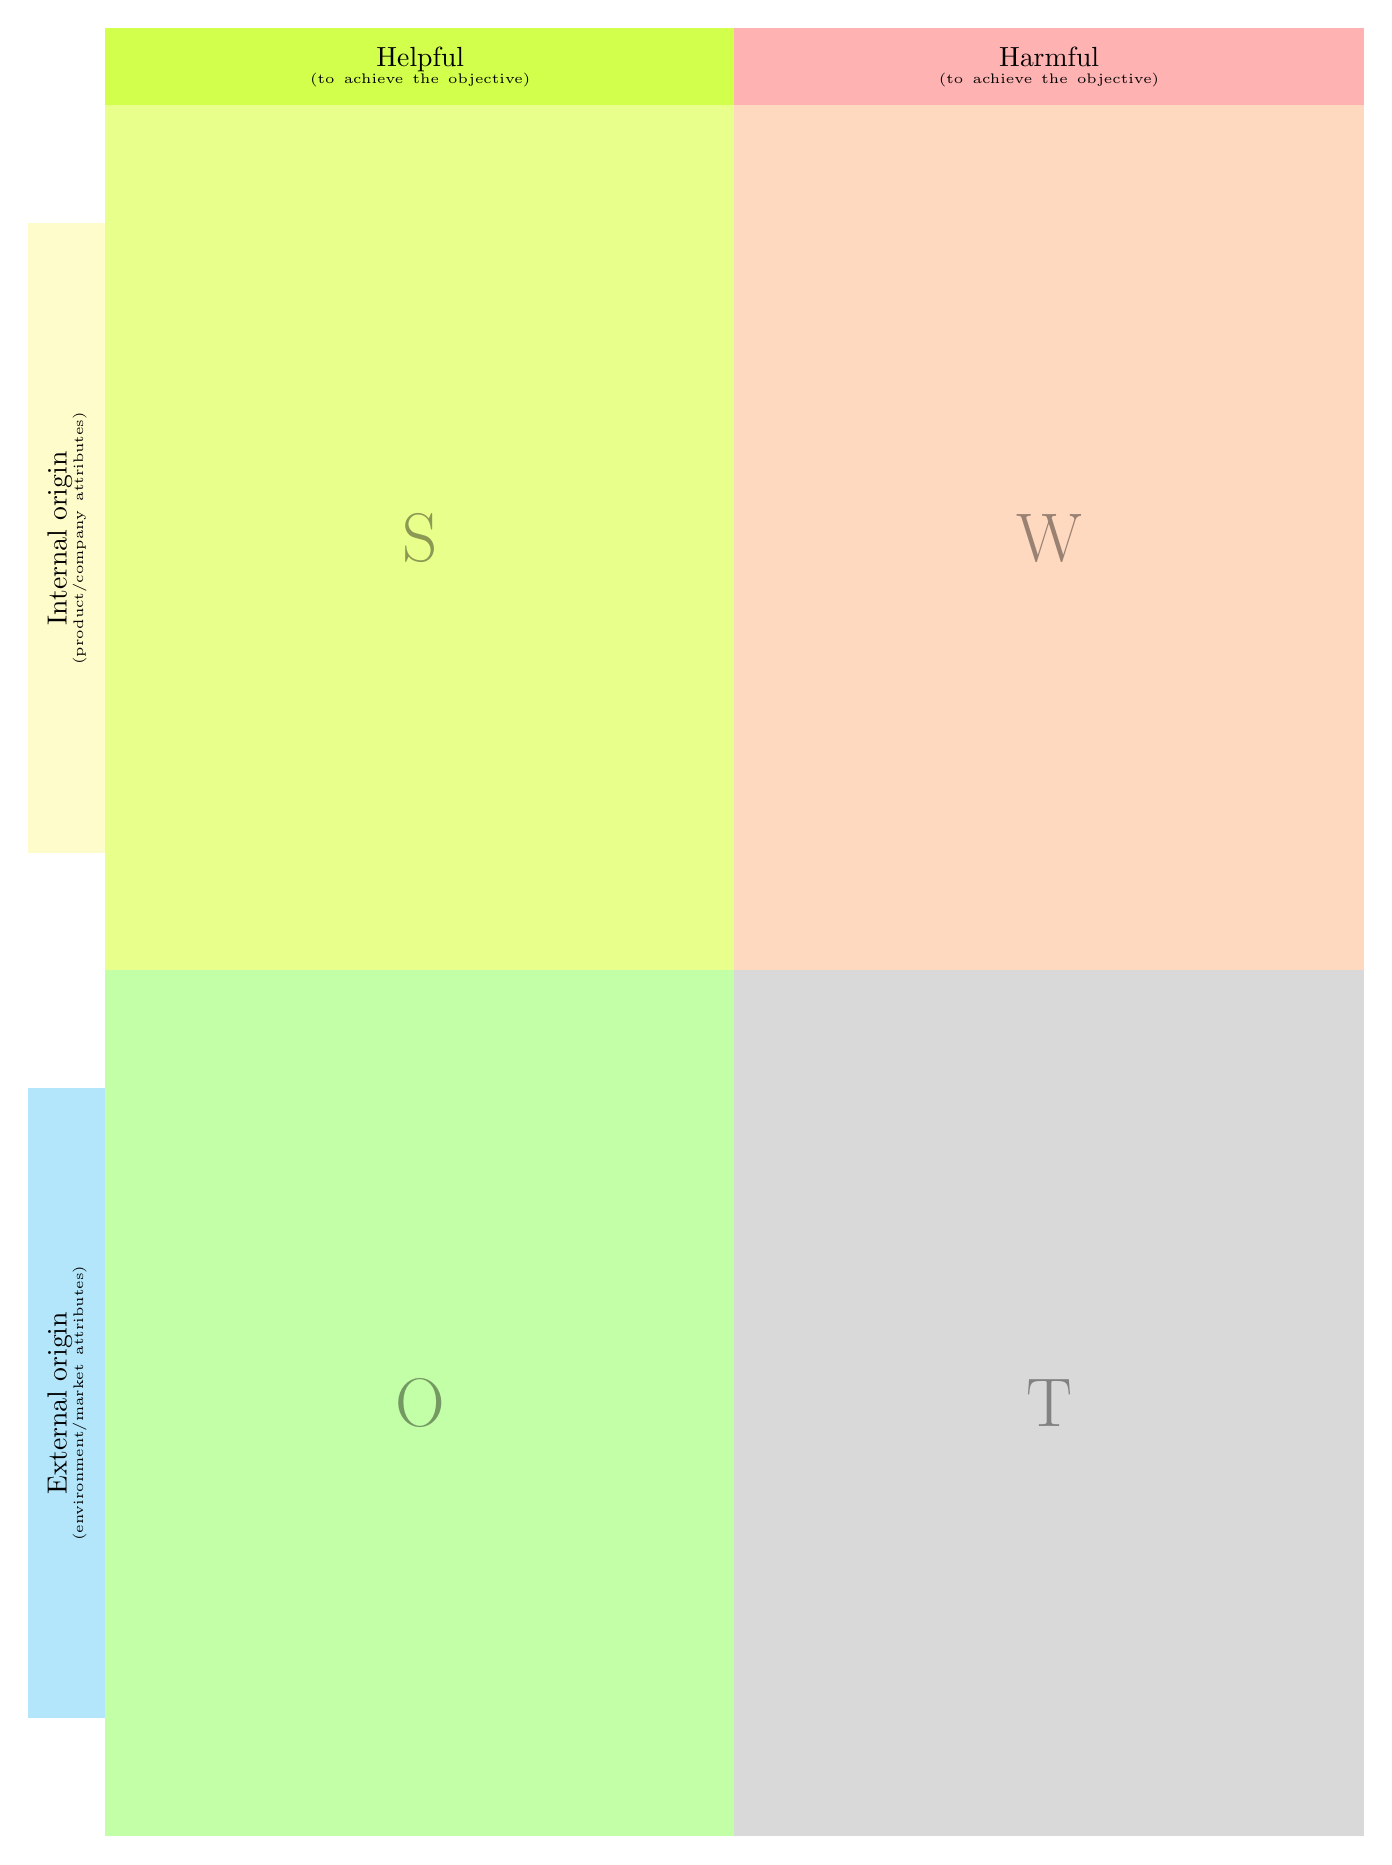
\begin{tikzpicture}[%
		%scale = 0.6, 
		%transform canvas={scale=0.6},
	    any/.style={minimum width=8cm,minimum height=11cm,%
	                 text width=7cm,align=center,outer sep=0pt},
	    header/.style={any,minimum height=1cm,fill=black!10},
	    leftcol/.style={header,rotate=90},
	    mycolor/.style={fill=#1, text=#1!60!black},
	]%
	\matrix (SWOT) [matrix of nodes,nodes={any,anchor=center},%
	                column sep=-\pgflinewidth,%
	                row sep=-\pgflinewidth,%
	                row 1/.style={nodes=header},%
	                column 1/.style={nodes=leftcol},
%	                row 1/.style={%
%						text width=4cm,
%            			minimum width=4cm,
%            			minimum height=7mm,	                
%	                },%
	                %column 1/.style={nodes=leftcol},%
	                inner sep=0pt]
	{%
	          &|[fill=helpful]| {\texta} & |[fill=harmful]| {\textb} \\
	|[fill=internal]| {\textcn} & |[mycolor=S]| \back{S} & |[mycolor=W]| \back{W} \\
	|[fill=external]| {\textdn} & |[mycolor=O]| \back{O} & |[mycolor=T]| \back{T} \\
	};%
	%\node[below right, any] at (SWOT-2-2.north west) {\Strengths};
	\node[any, anchor=center,transform shape] at (SWOT-2-2) {\Strengths};
	\node[any, anchor=center,transform shape] at (SWOT-2-3) {\Weaknesses};
	\node[any, anchor=center,transform shape] at (SWOT-3-2) {\Opportunities};
	\node[any, anchor=center,transform shape] at (SWOT-3-3) {\Threats};
	\end{tikzpicture}
%}